\documentclass[12pt]{article}
\usepackage{ctex}
\usepackage{graphicx}
\usepackage{indentfirst}

\title{第一周作业报告}
\author{佐藤拓未 20300186002}
\date{}

\begin{document}
	\maketitle
    \begin{center}
		\textbf{第一问}
    \end{center}
    利用MATLAB绘制$f(x)=\frac{1-\cos(x)}{x^2}$在$x\rightarrow0^+$时的图像,具体图像如下:
    \begin{figure}[h]
    	\centering
    	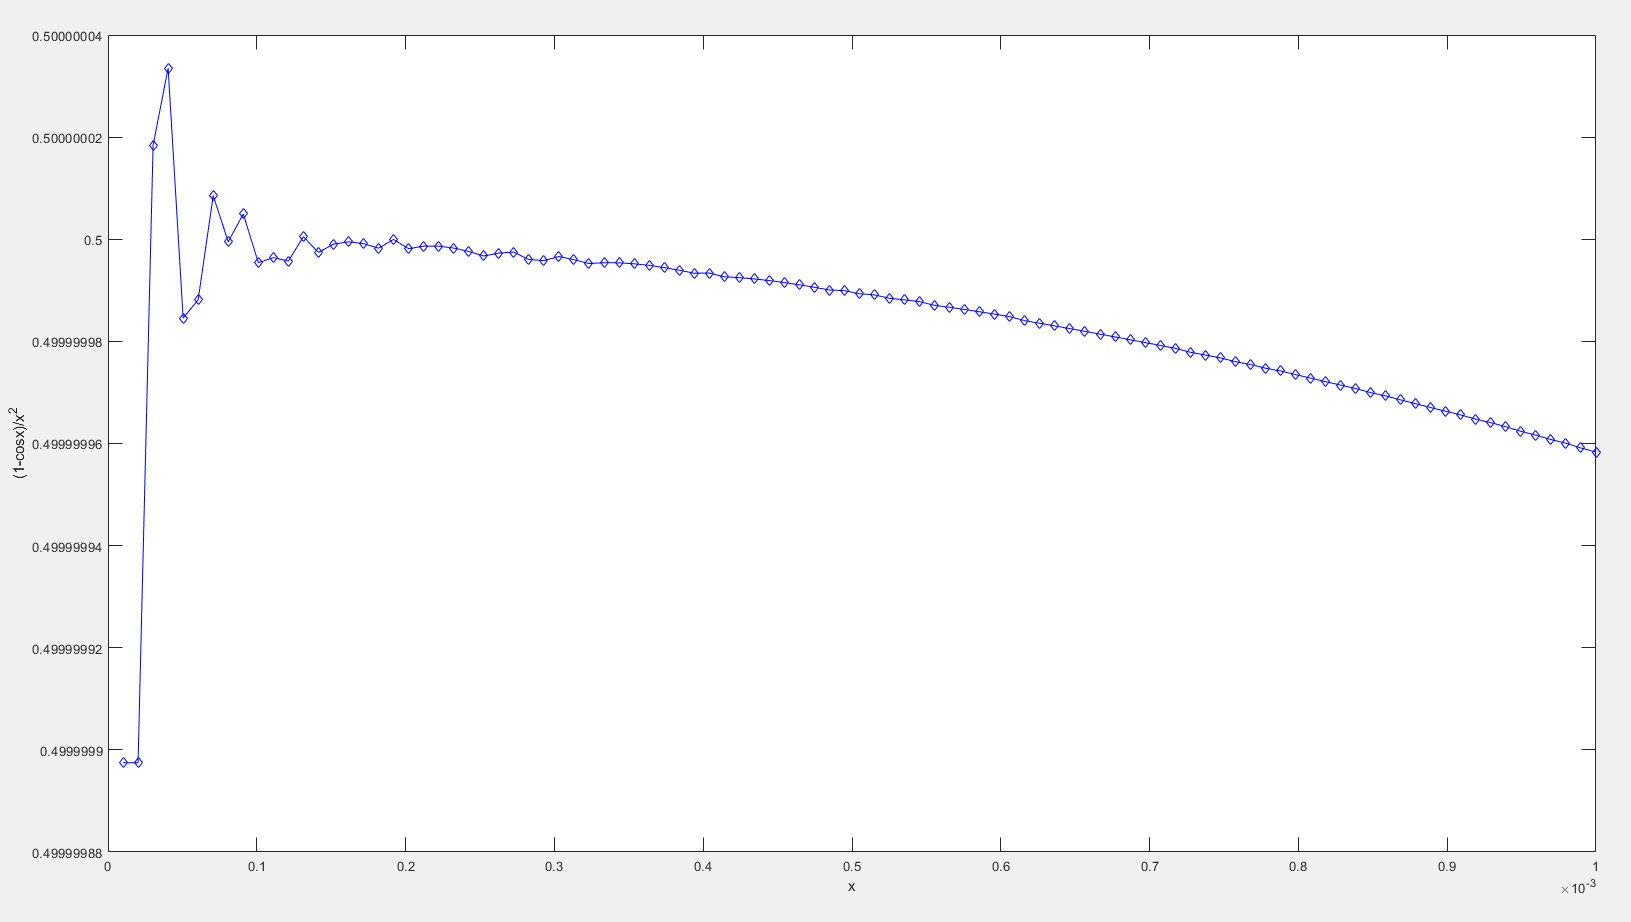
\includegraphics[width=1\textwidth]{图1}
    	\caption{在MATLAB中绘制出的函数图像}
    \end{figure}
  	\\
  	上图是$f$在$(0.001)$上100个等距节点上采样的函数值所得到的折线图像。
	\\
	但是可以知道$\lim\limits_{x\to0}\frac{1-\cos(x)}{x^2}=\frac{1}{2}$。
    \\
    \\
    
    \begin{center}
    	\textbf{第二问}
    \end{center}
	由递推公式$u_{n+2}-3u_{n+1}+2u_{n}=0$,以及$u_{100}=u_{99}=0.1$可以知道,${\forall}n:u_{n}=0.1$。
	\\
	在MATLAB中,考虑扰动$\epsilon=0.00001$,并令$v_{99}=u_{99}+\epsilon$以及$w_{99}=u_{99}-\epsilon$考虑反向递推,具体图像如下图所示:
	\begin{figure}[h]
		\centering
		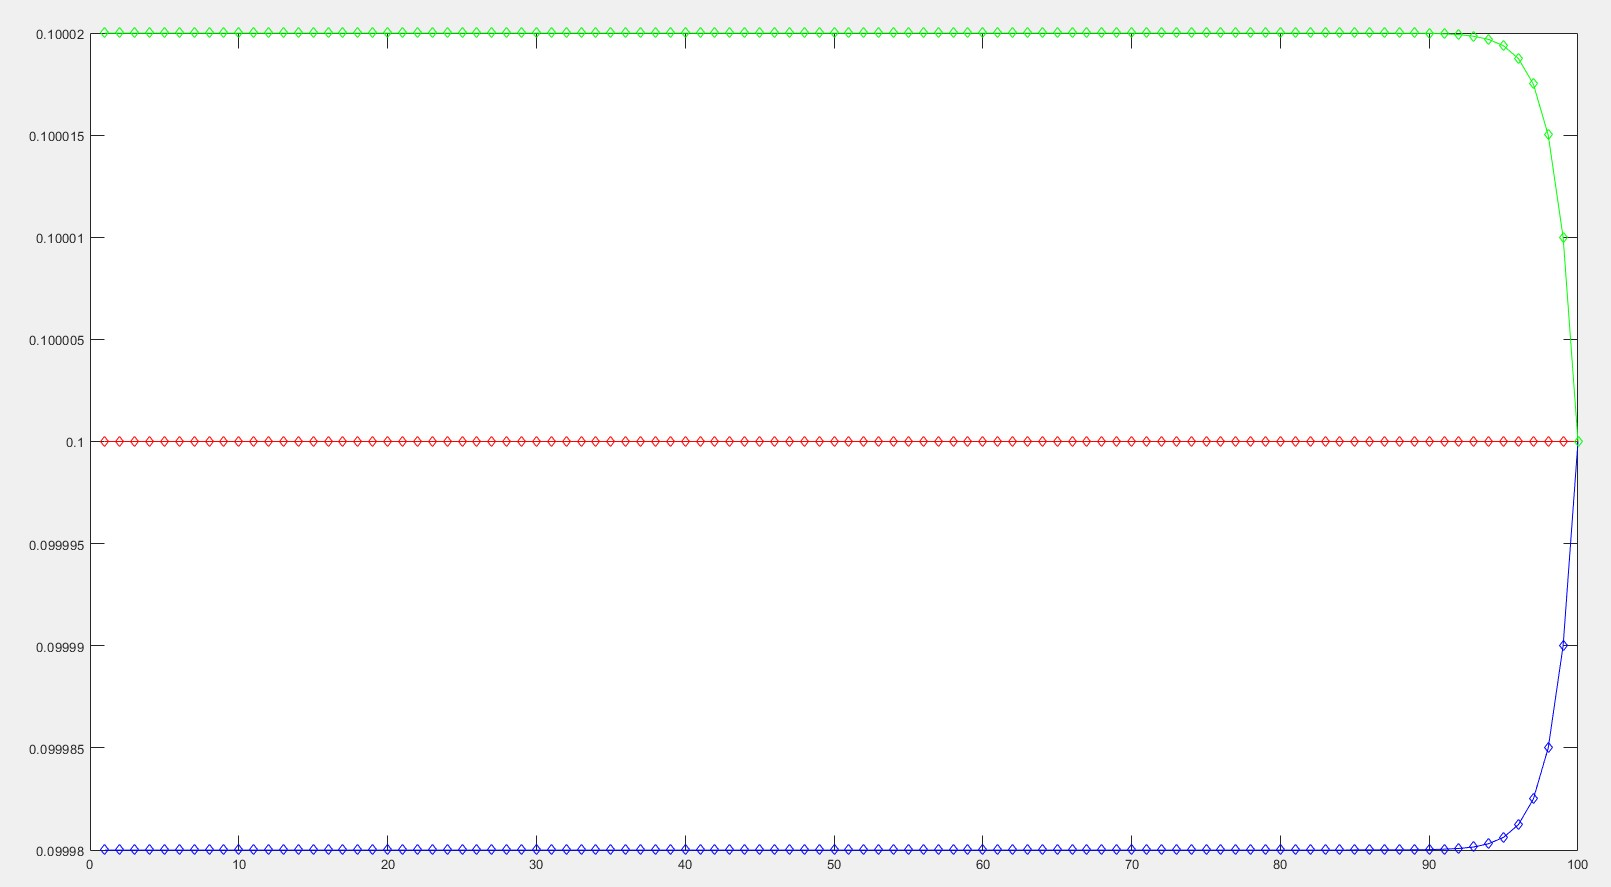
\includegraphics[width=1\textwidth]{图2}
		\caption{在MATLAB中绘制出的三个数列的对比}
	\end{figure}
	\\
	上图横坐标为数列下标,绿色对应于$\{v_n\}_{n=1}^{100}$,蓝色对应于于$\{w_n\}_{n=1}^{100}$,红色是恒为0.1的数列。
	\\
	可以发现最终$v_{1}\approx0.10002$,也有$w_{1}\approx0.09998$,以及它们与$u_{1}$的误差:$$\beta_{v}=\frac{\vert v_{1}-u_{1} \vert}{\vert u_{1} \vert}=0.0002$$ $$\beta_{w}=\frac{\vert w_{1}-u_{1} \vert}{\vert u_{1} \vert}=0.0002$$
	由于对$u_{99}$进行了扰动,因此通过反向迭代最终对$u_{1}$也产生了扰动,但总的来说其误差稳定。
	
\end{document}